%%%%%%%%%%%%%%%%%%%%%%%%%%%%%%%%%%%%%%%%%%%%%%%%%%%%%%%%%%%%%%%%%%%%%%%%%%%%%%%%%%%%%%%%%%%%%%%%
%                                                                                              %
%                             Definicao para a classe Artigo                                   %
%                                                                                              %
%%%%%%%%%%%%%%%%%%%%%%%%%%%%%%%%%%%%%%%%%%%%%%%%%%%%%%%%%%%%%%%%%%%%%%%%%%%%%%%%%%%%%%%%%%%%%%%%

\documentclass[portugues, brazil, a4paper,12pt]{article}
\bibliographystyle{plain}

%%%%%%%%%%%%%%%%%%%%%%%%%%%%%%%%%%%%%%%%%%%%%%%%%%%%%%%%%%%%%%%%%%%%%%%%%%%%%%%%%%%%%%%%%%%%%%%%
%                                                                                              %
%                       Pacotes a utilizar na compilacao do documento                          %
%                                                                                              %
%%%%%%%%%%%%%%%%%%%%%%%%%%%%%%%%%%%%%%%%%%%%%%%%%%%%%%%%%%%%%%%%%%%%%%%%%%%%%%%%%%%%%%%%%%%%%%%%

\usepackage[brazil]{babel}
\usepackage{graphicx}
\usepackage{geometry}
\usepackage[utf8]{inputenc}
\usepackage[T1]{fontenc}
\usepackage{algorithm}
\usepackage{color}
\usepackage{minted}
%\usepackage{algorithmic}
\usepackage[noend]{algpseudocode}
\usepackage{epstopdf}
\usepackage{hyperref}
\usepackage{todonotes}
\usepackage{amsmath}
\usepackage{verbatim}
\usepackage{gensymb}

\hypersetup{
    colorlinks,
    citecolor=black,
    filecolor=black,
    linkcolor=black,
    urlcolor=black
}



\makeatletter
\renewcommand{\paragraph}{\@startsection{paragraph}{4}{0ex}%
   {-3.25ex plus -1ex minus -0.2ex}%
   {1.5ex plus 0.2ex}%
   {\normalfont\normalsize\bfseries}}
\makeatother

\stepcounter{secnumdepth}
\stepcounter{tocdepth}

%%%%%%%%%%%%%%%%%%%%%%%%%%%%%%%%%%%%%%%%%%%%%%%%%%%%%%%%%%%%%%%%%%%%%%%%%%%%%%%%%%%%%%%%%%%%%%%%
%                                                                                              %
%                       Configuracao dos pacotes utilizados no doc.                            %
%                                                                                              %
%%%%%%%%%%%%%%%%%%%%%%%%%%%%%%%%%%%%%%%%%%%%%%%%%%%%%%%%%%%%%%%%%%%%%%%%%%%%%%%%%%%%%%%%%%%%%%%%

\geometry{a4paper,left=3cm,right=3cm,top=2.5cm,bottom=2.93cm}


%%%%%%%%%%%%%%%%%%%%%%%%%%%%%%%%%%%%%%%%%%%%%%%%%%%%%%%%%%%%%%%%%%%%%%%%%%%%%%%%%%%%%%%%%%%%%%%%
%                                                                                              %
%                             Capa do relatorio tecnico                                        %
%                                                                                              %
%%%%%%%%%%%%%%%%%%%%%%%%%%%%%%%%%%%%%%%%%%%%%%%%%%%%%%%%%%%%%%%%%%%%%%%%%%%%%%%%%%%%%%%%%%%%%%%%

\begin{document}

\begin{titlepage}

  \vfill

	\begin{figure}[H]
	\centering
		
\includegraphics[scale=0.15]{img/logo-ufop.jpg}
	\end{figure}

  \vfill

  \begin{center}
    \begin{Large}
      \textbf{UNIVERSIDADE FEDERAL DE OURO PRETO}
    \end{Large}
  \end{center}

  \begin{center}
    \begin{large}
      \textbf{Mestrado em Ciência da Computação} \\[1.4cm] 
    \end{large}
  \end{center}

  \vfill

  \begin{center}
    \begin{large}
      \textbf{Especificação Sistêmica de Carro Robô Seguidor de Linha com Sistema Avançado Utilizando Controle Proporcional}
    \end{large}
  \end{center}

  \vfill

  \begin{center}
    \begin{large}
      Autor: \\
		Rodolfo Labiapari Mansur Guimarães - \url{rodolfolabiapari@decom.ufop.br}
    \end{large}
  \end{center}

	\vfill

  \begin{center}
    \begin{large}
      Professor: \\
      Ricardo Augusto Rabelo Oliveira - \url{rrabelo@gmail.com}
    \end{large}
  \end{center}

  \vfill

  \begin{center}
    \begin{large}
      Ouro Preto - MG \\
      \today \\
    \end{large}
  \end{center}

\clearpage
\tableofcontents 
\end{titlepage}

%%%%%%%%%%%%%%%%%%%%%%%%%%%%%%%%%%%%%%%%%%%%%%%%%%%%%%%%%%%%%%%%%%%%%%%%%%%%%%%%%%%%%%%%%%%%%%%%
%                                                                                              %
%                               Introducao ao trabalho                                         %
%                                                                                              %
%%%%%%%%%%%%%%%%%%%%%%%%%%%%%%%%%%%%%%%%%%%%%%%%%%%%%%%%%%%%%%%%%%%%%%%%%%%%%%%%%%%%%%%%%%%%%%%%

\section{Introdução}
	Atualmente é possível construir Carro Robô Seguidor de Linha utilizando poucos componentes, e com poucas linhas de programação.
	
	É possível encontrar facilmente em sites de venda de eletrônicos, kits de sensores e atuadores de baixo custo prontos para serem acoplados à placa de prototipagem e assim, a construção de um carro seguidor.
	
	O desenvolvimento do sistema controlador também segue o mesmo princípio de facilitação de uso. Utilizando uma plataforma de prototipagem tal como Arduino, é possível escrever o controle de um carro seguidor com poucas linhas de instruções. Isso pode ser levado como um desafio até para crianças e adolescentes com criatividade e entusiasmo para desenvolver um sistema completo e funcional como incentivo à robótica.
	
	Entretanto, o que diferencia de grandes competidores de amadores é o algoritmo de controle do carro. Algoritmos com controles simples funcionarão e completarão a prova, mas terão grande dificuldade. O que diferencia carros simples à complexos e velozes seguidores de linha não são seus componentes, organização e a precisões desses, mas sim a adaptação de seu controle. Com isso, o objetivo deste trabalho é especificar um carro seguidor de linha onde ele deverá possuir todos os equipamentos necessários para a conclusão de seu objetivo além de uma adaptação na avaliação e atuação de seus sensores para que este possa obter melhores resultados usando cálculos matemáticos mais elaborados a seu favor como Controle Proporcional.
	
	Na Seção \ref{sec:rt} será feito uma introdução às definições matemáticas dos temas abordados no texto. Nesta Seção encontra-se todos os detalhes técnico-matemáticos para o compreendimento do trabalho. Na Seção \ref{sec:elementosProjeto} é descrito brevemente sobre os equipamentos utilizados no projeto para seu funcionamento. Por fim, na Seção \ref{sec:implementacao} é descrito um pseudocódigo do procedimento proposto.

\section{Referencial Teórico} \label{sec:rt}
	
	\subsection{Equação Diferencial Linear}
		Equações Diferenciais Lineares são equações que suas soluções podem ser somadas a fim de produzir uma nova solução. 
		
		É considerada linear quando satisfaz as características de que cada coeficiente a $a_{n}$ e o termo de não-homogeneidade só dependem da variável independente, no caso $x$; e a variável dependente, no caso $y$, e suas derivadas são de primeiro grau. Assim, ela deve representar a seguinte forma
		
		\begin{equation}
			f(x) = a_{n}(x)\frac{d^{n}y}{dx^{n}} + a_{n-1}(x)\frac{d^{n-1}y}{dx^{n-1}} + \cdots +  a_{1}(x)\frac{dy}{dx} + a_0(x)y
		\end{equation}
		
		\begin{comment}
		
		No uso para problemas que utilizam Controle Proporcional descrito no Seção \ref{sec:controle_proporcional}, basta desligar todas as derivadas e integrais da equação obtendo
		
		\begin{equation}
		f(x) = a_{n}(x) + a_{n-1}(x) + \cdots +  a_{1}(x) + a_0(x)y
		\end{equation}
		
		\end{comment}
		
	\subsection{Controlador Proporcional} \label{sec:controle_proporcional}
	
		\subsubsection{Visão Geral}
			A teoria de controladores proporcionais se baseiam em sistemas realimentados. Tais podem ser divididos em basicamente três partes sendo elas:
			\begin{itemize}
				\item Sistema a ser controlado;
				\item Controlador (também conhecido como compensador); e
				\item Realimentação.
			\end{itemize}
			
			O sistema a ser controlado é constituído por atuadores capazes de efetuar as ações necessárias. Os outros dois elementos têm como finalidade fazer com que o desempenho do sistema possua estabilidade e opere com certa precisão e agilidade, seguindo as especificações uma vez estabelecidas. Uma vez estabelecido como o sistema deverá ser desenvolvido, os controladores e sua realimentação serão item essencial para que o processo ocorra de forma estável. Tudo isso pode ser observado no diagrama exibido na Figura \ref{fig:estrutura_sistema_controle}.
			
			\begin{figure}[H]
				\centering
				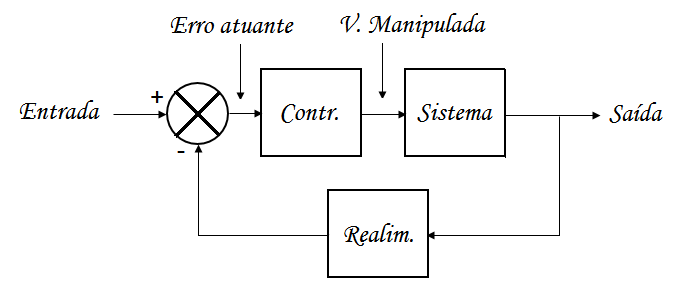
\includegraphics[width=\linewidth]{img/cp-realimentacao.png}
				\caption{Estrutura de Sistema de Controle Geral.}
				\label{fig:estrutura_sistema_controle}
			\end{figure}
			
			A realimentação é o ponto chave para a diferenciação de sistemas controladores comuns. Um sistema de controle realimentado compara, instantaneamente, o valor de saída anterior, com o valor de referência existente na entrada do sistema como os sensores. O resultado desta comparação é o centro de toda adaptabilidade estudada e é denominado erro atuante. Este é levado ao controlador, que produz o chamado sinal de controle, cuja função resume-se em reduzir o desvio entre a saída e o sinal desejado. Como o nome sugere, em um controlador proporcional a saída do mesmo, também conhecido como sinal de controle (ou ação de controle), é diretamente proporcional ao sinal de erro, ou seja, ao erro atuante.
			
			Sabendo-se em da proporcionalidade direta entre o sinal de controle e o sinal de erro, é possível afirmar que
			
			
			\begin{equation}
				a(t) \propto e(t)
			\end{equation}
			
			onde o controle é diretamente proporcional à seu erro.
			
			Entretanto, não é possível realizar operações matemáticas exatas com o sinal de proporção da fórmula. Par isso, deve-se admitir então uma constante de proporcionalidade entre as mesmas. Esta possui o nome de ganho proporcional e é representado pela variável $f$. Sendo assim
			
			\begin{equation}
				a(t) = f * e(t) \label{eq:formula_geral}
			\end{equation}
			
			Dessa forma, o sistema matemático mostrado na Equação \ref{eq:formula_geral} poderá ser representado pelo diagrama exibido na Figura \ref{fig:sistema_dominio_tempo}.
			
			\begin{figure}[H]
				\centering
				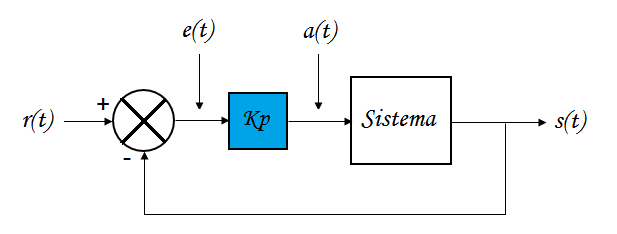
\includegraphics[width=\linewidth]{img/cp-diagrama_geral.png}
				\caption{Sistema no Domínio do Tempo Geral.}
				\label{fig:sistema_dominio_tempo}
			\end{figure}
			
			Sendo assim, como fórmula final, temos
			
			\begin{equation}
				a(t) = f * (r(t) - s(t))
			\end{equation}
			
			onde $a(t)$ é a atuação, $e(t)$ representa o erro, $ r(t) $ é o valor de início de execução de controle e $ s(t) $ é saída do controle. Todos representando o valor no tempo $t$.
	
	\subsection{Modelamento Teórico-Matemático}
		\subsubsection{Definições}
			%https://syclops.wordpress.com/2011/08/06/part-2-line-following-robot-code-guideline-arduino-using-pid/
			Para iniciar a discussão sobre sistema de controle proporcional, primeiramente será definido os termos utilizados.
			
			\begin{description}
				\item[\textit{Alvo:}] É a posição que desejamos que o carro esteja em relação à faixa, ou seja, centralizado respeitando a devida linha.
				
				\item[\textit{Erro:}] Diferença entre a posição atual e o \textit{Alvo}. Pode ser qualquer valor no conjunto dos ${\rm I\!R}$.
				
				\item[\textit{Proporção:}] Fator que determinará quão distante o carro está da linha. Por exemplo são as proporções: `\textit{para a esquerda}',  `\textit{para a direita}', `\textit{para a extrema esquerda}', `\textit{pouco para a direita}', etc. É representado pela constante de variação $ K_p $.
				
				\item[\textit{Integral:}] Proporciona o erro acumulado sobre o tempo corrido. Isso significa que este irá informar se o carro vem estando na linha nos últimos momentos ou não. Representada pela constante de variação $ K_i $.
				
				\item[\textit{Derivada:}] Taxa no qual exibe a oscilação do robô sobre a linha, representada pela constante de variação $ K_d $.
			\end{description}
			
			Ambos \textit{Integral} e \textit{Derivada} utilizam o valor \textit{Proporção}.
		
			O procedimento de execução é baseado no seguinte pseudocódigo:
			\begin{enumerate}
				\item Realiza o cálculo inicial da posição atual.
				
				\item Calcula o erro baseado na posição atual.
				
				\item Ele então comandará os motores para fazer uma girada:
				\begin{itemize}
					\item Brusca caso o erro for grande; ou
					\item Leve caso o erro for pequeno.
				\end{itemize}
				Basicamente, a magnitude do giro tomado é proporcional ao \textit{erro}.
				
				\item Repete os passos até completar o objetivo.
			\end{enumerate}
			
			Com esses passos, saímos de um controle simples para um Contro Proporcional mais eficaz. 
			
			Mesmo se depois desses passos o valor de \textit{erro} não decrementar ou decrementar de forma bem lenta, ao realizar o passo 4, o controlador fará uma nova avaliação incrementando a magnitude de conserto de posição realizando novamente de forma mais brusca a tentativa de posicionar o carro novamente à posição centralizada. Esse processo só é possível por causa do Controle Integral. O efeito de redução de oscilação por tempo é trabalho pelo Controle Derivativo.
	
	%\subsection{Modelamento Teórico-Matemático do Sistema}
		O Controlador Proporcional Integral-Derivativo, também chamado de Controlador PID, é uma metodologia de cálculo de controle de processo que une várias outras menores. Utiliza de teorias como as Ações Derivativa (Controle PD), Integral (Controle PI) e Proporcional (Controle P).
		
		Estes quatro modos de controle, incluindo PID, são também designados de ações de controle, cada uma delas reagindo de forma distinta ao erro presente nos sistemas. O controle:
		
		\begin{itemize}
			\item Proporcional: ajusta a variável de controle de forma proporcional ao erro;
			\item Integral: ajusta a variável de controle baseando-se no tempo em que o erro acontece;
			\item Derivativo: ajusta a variável de controle tendo como base a taxa de variação do erro; e
			\item A combinação destes tipos de controle forma o controlador PID.
		\end{itemize}
		
		São amplamente utilizados em situações que se baseiam em controladores eletrônicos chamados ``\textit{single-loop}''.
		
		Como ele é formado por todos os outros controles, será descrito brevemente cada um deles.
		
	\subsubsection{Teoria de Controle Proporcional (P)} \label{sec:P}
	Produz um sinal de saída que é proporcional à parâmetro do erro 
	
	\begin{equation}
	P_{\mathrm {saida} }=K_{p}\,{e(t)}
	\end{equation}
	
	onde
	
	\begin{description}
		\item[$ e(t) $\textit{:}] Erro.
		
		\item[$ K_p $\textit{:}] Constante relativa à proporção.
	\end{description}
	
	Esse método possui a propriedade de eliminar as oscilações do sinal de saída. Para tal, o sistema permanece sempre ligado e o sinal de saída é diferente de zero.
	
	\subsubsection{Teoria de Controle Proporcional Integral (PI)} \label{sec:PI}
	Gera um sinal de saída que é proporcional à magnitude e à duração do erro, ou seja, ao erro acumulado. Isso fornece uma alternativa para acelerar a resposta do sistema, permitindo-o chegar ao valor de referência mais rapidamente.
	
	\begin{equation}
	I_{\mathrm {saida} }=K_{i}\int _{0}^{t}{e(\tau )}\,{d\tau }
	\end{equation}
	
	onde 
	
	\begin{description}
		\item[$ K_i $\textit{:}] Constante de ganho integral.
		
		\item[$ \tau $\textit{:}] Tempo integral.
	\end{description}
	
	A ação integral corrige o valor da variável manipulada em intervalos regulares (representado como $ \tau $). Ele é definido como o inverso do ganho integral. 
	
	\subsubsection{Teoria de Controle Proporcional Derivativo (PD)} \label{sec:PD}
	Resulta num sinal de saída que é proporcional à velocidade de variação do erro.
	
	\begin{equation}
	D_{\mathrm {saida} }=K_{d}{\frac {de(t)}{dt}}
	\end{equation}
	
	onde 
	
	\begin{description}
		\item[$ K_d $\textit{:}] Constante de ganho derivativo.
	\end{description}
	
	Ela fornece uma correção antecipada do erro, diminuindo o tempo de resposta e melhorando a estabilidade do sistema. Atua em intervalos regulares, chamado tempo derivativo.
	
	
	\subsubsection{Teoria de Controle Proporcional Integral-Derivativo (PDI)} \label{sec:PID}
	Assim, fazendo um casamento de todos os controles P, PI, PD, ditos nas Seções \ref{sec:P}, \ref{sec:PI}, \ref{sec:PD}, temos a seguinte fórmula
	
	\begin{equation} \label{eq:PID}
	u(t) = \underbrace{K_p e(t)}_{P} + \underbrace{K_i \int_{0}^{t} e(\tau) d\tau}_{PI} + \underbrace{K_d\frac{de(t)}{d(t)}}_{PD}
	\end{equation}
	
	onde
	
	\begin{description}
		\item[$ K_p $\textit{:}] Ganho Proporcional.
		
		\item[$ K_i $\textit{:}] Ganho Integral.
		
		\item[$ K_d $\textit{:}] Ganho Derivativo.
		
		\item[$ e $\textit{:}] Erro.
		
		\item[$ t $\textit{:}] Tempo.
		
		\item[$ \tau $\textit{:}] Tempo integral.
	\end{description}
	
	Aplicando a transformada de Laplace na Equação \ref{eq:PID}, obtemos:
	
	\begin{equation}
	L(s)=K_{p}+\frac{K_{i}}{s}+K_{d}s
	\end{equation}
	
	sendo
	
	\begin{description}
		\item[$ s $\textit{:}] Frequência complexa.
	\end{description}
	
	
\section{Elementos do Projeto} \label{sec:elementosProjeto}

	\subsection{Microcontrolador}
		Microcontrolador utilizado para este trabalho é o NodeMCU. É um plataforma IoT\footnote{\textit{Internet of Things}, ou seja, internet das coisas.} \textit{open-source}. 
		
		Como esperado de um microcontrolador para IoT o sistema possui integrado um componente de comunicação Wi-Fi para troca de dados. Utiliza linguagem de \textit{script} Lua desenvolvida por brasileiros.
		
		Suas especificações são uma CPU ESP8266 possuindo 128 KB de memória, 4 MB de armazenamento e suporta o sistema operacional chamado XTOS. Permite comunicação pelo Wi-Fi e USB onde também é energizada. Possui um total de 10 pinos de entrada e saída de propósito geral (GPIO) onde suportam funções como PWM, comunicação I$ ^2 $C e 1-wire. Além da antena Wi-Fi, possui também um conversor USB-TTL para comunicação serial.
		
		Seus microprocessadores podem ser facilmente ligados à um computador e também utilizado a IDE Arduino. A Figura \ref{fig:eq-nodemcu} exibe um esquemático de seu protótipo.
		
		\begin{figure}[t]
			\centering
			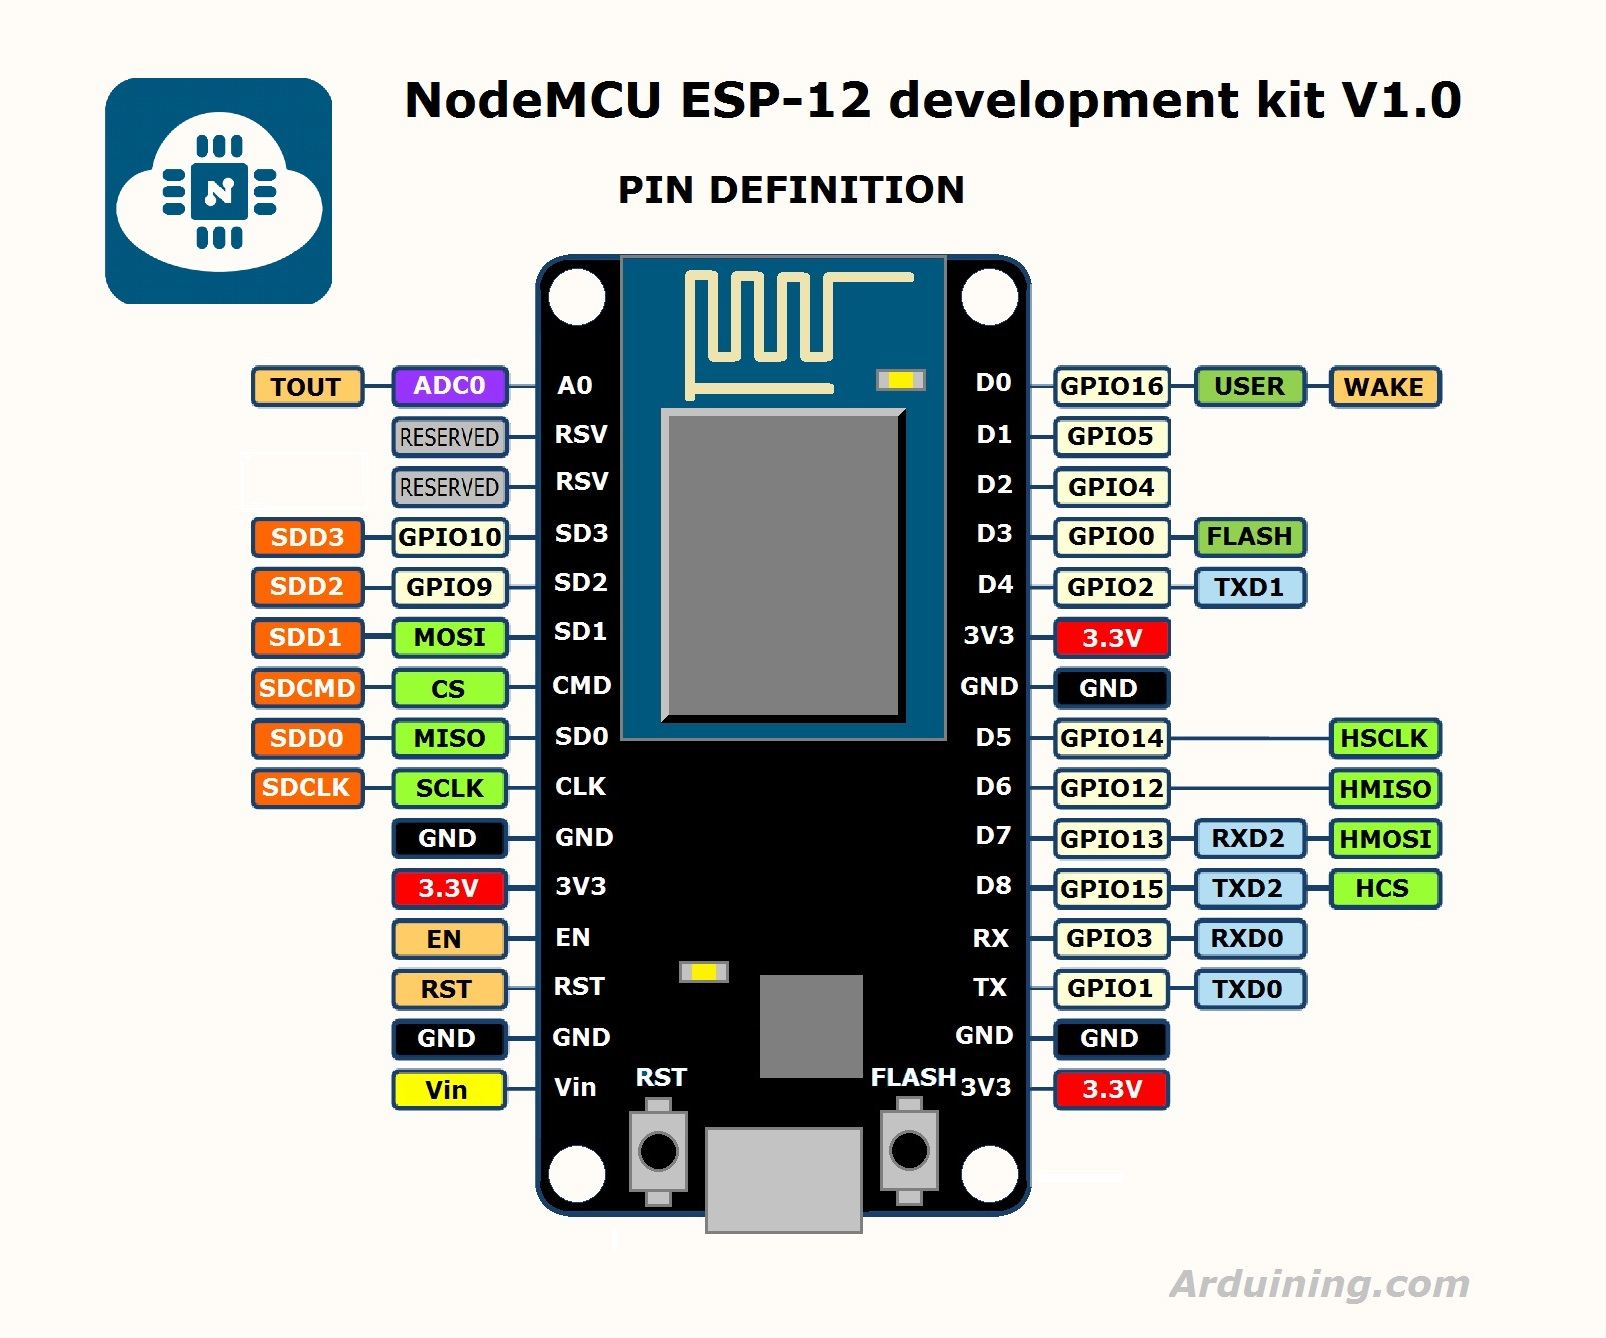
\includegraphics[width=0.9\linewidth]{img/eq-nodemcu.jpg}
			\caption{O Microcontrolador NodeMCU e seus Componentes e I/O.}
			\label{fig:eq-nodemcu}
		\end{figure}
		
		Sua programação pode ser feita por diversas maneiras. As duas principais são utilizando um terminal serial para envio de comandos diretamente à placa usando a porta USB do controlador. Para isso, deve-se configurar a comunicação serial para 9600 \textit{baud-rate}. Ao iniciar o controlador, já iniciará informações de comunicação. Feito isso, já é possível enviar comandos ao controlador. Outra forma é utilizando programas para envio de dados até a placa. Eles realizarão toda a `interfaceação' do desenvolvedor com a placa e um exemplo deles é a IDE Arduino.
		
		Como ela possui placa de comunicação Wi-Fi e um controlador poderoso, é possível também transformá-la num \textit{Web Service} para que realize toda a comunicação sem fio.

	\subsection{Energização}
		Sua energização será realizada por meio de fonte externa. Isso é necessário pois o sistema completo possui vários componentes que necessitam de uma fonte de energia estável e constante para não afetar no desempenho e também pelo fato do controlador não conseguir fornecer mais que 3.3V e 12mA em suas saídas GPIO. Qualquer valor fora deste intervalo pode gerar em não corretude do sistema, inclusive danificação.
		
		Utilizar uma fonte por meio da interface USB não seria suficiente para energizar todos os atuadores e sensores do sistema justificando assim o uso da fonte externa.
	
	\subsection{Sensores}
		Para o carro, será utilizado somente um único tipo de sensor para seu funcionamento, sendo este será o sensor fototransistor. Em sua superfície, existirá um LED que fará a iluminação da área no qual refletirá sobre a superfície e chegará até o sensor fototransistor. Como o seguidor de linha move sobre dois tipos de superfície (branca e preta), é possível identificar quando ele sairá da direção correta. Essa ideia melhor visualizada com a Figura \ref{fig:ft}.
		
		\begin{figure}[H]
			\centering
			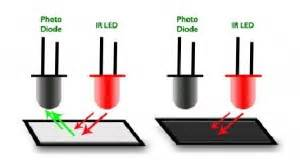
\includegraphics[width=0.4\linewidth]{img/eq-fototransistor.jpg}
			\caption{Sensor Fototransistor.}
			\label{fig:ft}
		\end{figure}
		
		O projeto utilizará não somente dois sensores mas uma série deles, posicionados logo à extremidade da faixa de direção como é exibido na Figura \ref{fig:dois_sensores}.
		
		\begin{figure}[H]
			\centering
			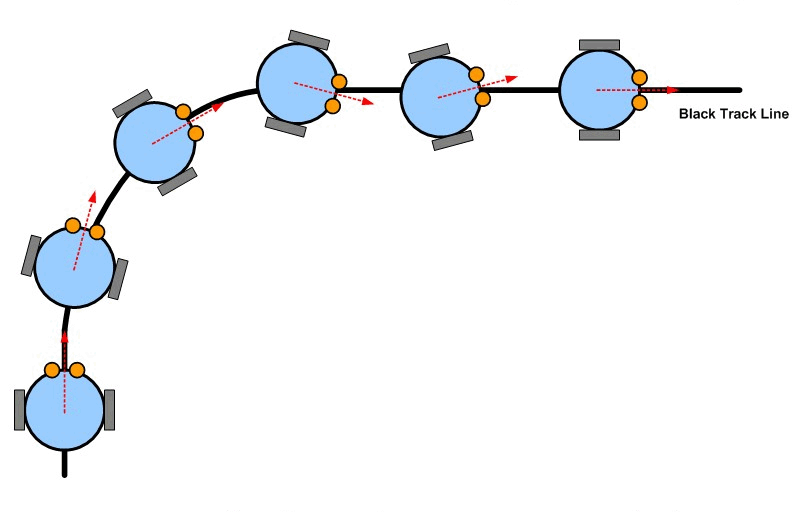
\includegraphics[width=0.9\linewidth]{img/eq-line-tracking.png}
			\caption{Posição dos Sensores. Exemplo utilizando dois sensores.}
			\label{fig:dois_sensores}
		\end{figure}
	
		Utilizando uma série de sensores, cada sensor será responsável por avaliar se o carro saiu da linha original. Quanto mais à extremidade a faixa estiver em relação à série de sensores, maior será o erro dela e assim, a consequente uma correção mais rápida. Quanto maior a quantidade de arranjo de sensores melhor será a performance do carro pelo motivo que mais sensores representarão melhor o nível do erro. Por este motivo, será utilizado seis sensores, posicionando três em cada extremidade da faixa. Eles serão dispostos o mais próximo possível de seu adjacente pois a resolução de operação será melhor do que distâncias grandes como três centímetros ou mais. Um exemplo com 8 sensores é exibido na Figura \ref{fig:sensores_series}. 
	
		\begin{figure}
			\centering
			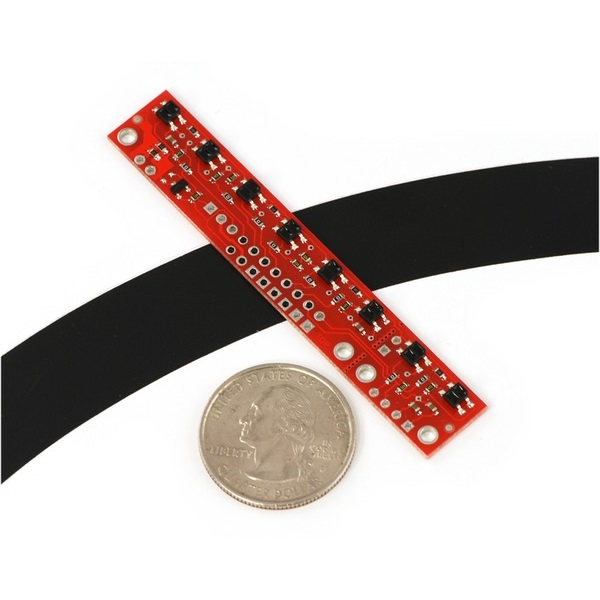
\includegraphics[width=0.7\linewidth]{img/eq-sensores_series.jpg}
			\caption{Sensores em série.}
			\label{fig:sensores_series}
		\end{figure}

	
		O carro andará numa velocidade máxima fixa em um valor. Quando algum de seus sensores perceber que o carro saiu da linha, a fórmula de correção de direção será acionada para avaliar os dados dos sensores e assim verificar os procedimentos a serem realizados nos atuadores para que o carro volte a operar normalmente na direção correta em cima da faixa. Nesta parte que existe o grande diferencial deste trabalho proposto.

		Utilizando controle simples, sem realimentação, é possível perceber que seu erro após à primeiro desvio será grande e sua forma de conserto fará com que ele aumente ainda mais sua margem de erro. isso causará grande distúrbio em seu movimento criando assim um padrão geométrico construído por uma sequência de segmentos lineares alternados quanto à direção, formando linhas quebradas com alternância de ângulos salientes e reentrantes como mostrado na Figura \ref{fig:trajeto2}.
		
		\begin{figure}[H]
			\centering
			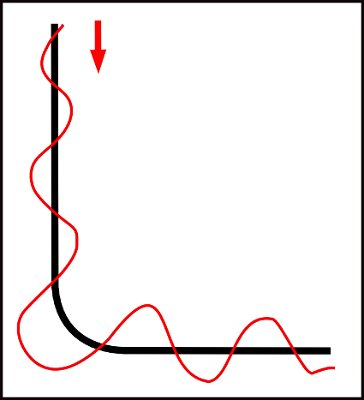
\includegraphics[width=0.5\linewidth]{img/trajeto2.jpg}
			\caption{Seguidor de Linha comum.}
			\label{fig:trajeto2}
		\end{figure}
	
		Esse movimento oscilatório faz com que o carro gaste tempo em completar sua tarefa de percorrer a linha e também energia, item essencial para sistemas embarcados.
	
		Já utilizando o controle proposto é possível que este padrão seja decrementado ao ponto de tornar o movimento do carro mais suave e portanto seu trajeto mais conciso quanto à linha do trajeto. O resultado esperado é exibido na Figura \ref{fig:trajeto3}.
	
		\begin{figure}[H]
			\centering
			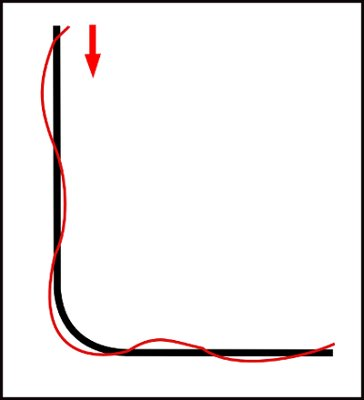
\includegraphics[width=0.5\linewidth]{img/trajeto3.jpg}
			\caption{Seguidor de Linha utilizando Controle Proporcional.}
			\label{fig:trajeto3}
		\end{figure}
	
		Este trajeto faz com que seus movimentos sejam mais suaves, estáveis, ágeis e eficientes em relação ao mostrado na Figura \ref{fig:trajeto2}.
		
		
	\subsection{Atuadores}
		O sistema possuirá duas unidades de motores atuadores.
		
		Os motores serão do tipo de Corrente-Contínua, propriedade física que não permite o cálculo exato de distância e velocidade do equipamento sem a utilização de sensores de marcação de passo. Para isso, será utilizado vários sensores para captação de dados do ambiente (que no caso será a faixa a ser seguida) e processado para enviar dados de controle aos atuadores para o carro manter o mais centralizado à faixa.
		
		Eles serão acoplados à \textit{board} utilizando um \textit{shield} intermediário entre o microcontrolador e os motores. Inicialmente, serão acionados em uma velocidade máxima $ s $. Quando o carro perceber que necessita de uma correção na direção, independente do grau dela, o motor responsável por corrigir o erro será decrementado em sua velocidade, tentando aproximar da direção desejada. Esse processo repetirá enquanto o carro não completar sua meta de trafegar pelo circuito todo.
		
		Tal \textit{shield} realizará o processo de interface de controle e energização dos motores criando assim um sistema estável. Seu nome é L293DD e possui suporte total para interface de pinos NodeMCU. Seu sistema de operação utiliza Ponte-H dupla e com isso é possível controlar até dois motores além de conectores para seleção de interface serial UART, SPI, e entrada analógica, além de conexões para habilitar as opções de \textit{Enable} e \textit{Reset} do microcontrolador. Ele pode ser visto por meio da Figura \ref{fig:eq-motor_shield}.
		
		\begin{figure}[H]
			\centering
			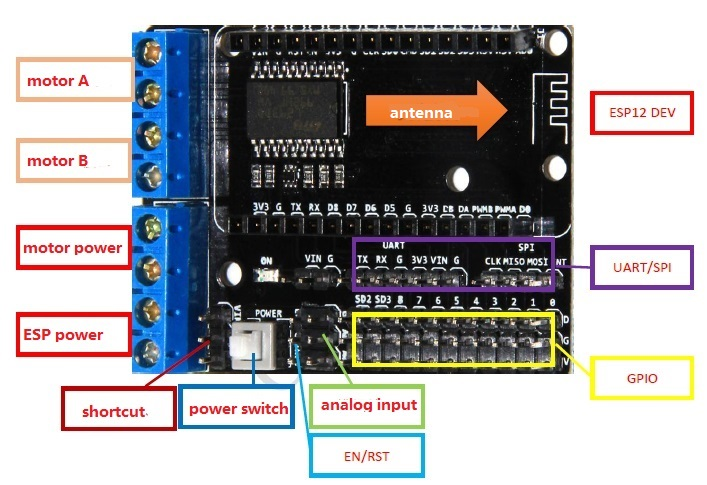
\includegraphics[width=0.9\linewidth]{img/eq-motor_shield.jpg}
			\caption{Motor \textit{Shield} a ser Utilizado.}
			\label{fig:eq-motor_shield}
		\end{figure}
		

\section{Implementação} \label{sec:implementacao}
	Aqui será descrito uma representação de como será a implementação de toda a teoria descrita neste trabalho. Assim, de forma geral, teremos o seguinte algoritmo implementado para tratamento dos valores obtidos dos sensores e ajuste da rotações dos motores. 
	
	\begin{algorithm}[H]
		\caption{Controle Proporcional de Correção de Angulação}\label{euclid}
		\begin{algorithmic}[1]
			\Procedure{proportional\_control}{$position, set\_point, \Delta, \int, last\_\Delta, y', \Phi $}
				\State $ \Delta \gets position - set\_point$
				\State $ \int \gets \int + \Delta$
				\State $ y' \gets \Delta - last\_\Delta $
				\State $ \Phi \gets \Delta * K_p + \int * K_i + y' * K_d $
			\EndProcedure
		\end{algorithmic}
	\end{algorithm}

	onde:
	\begin{description}
		\item[\textit{position:}] Posição atual do carro.
		
		\item[\textit{set\_point:}] Ponto central onde encontra-se a faixa.
		
		\item[$ \Delta $\textit{:}] Representa o erro proporcional da posição atual contra o ponto central da faixa.
		
		\item[$ \int $\textit{:}] Representa o acúmulo de erro atual.
		
		\item[$ last\_\Delta $\textit{:}] Representa o erro proporcional da posição da iteração passada.
		
		\item[$ y' $\textit{:}] Retêm a diferença entre os erros atual e da iteração anterior.
		
		\item[$ \Phi $\textit{:}] Correção a ser realizada nesta iteração.
	\end{description}
	
	Como é de se esperar, a correção proporcional $ \Phi $ será aplicada à velocidade motor para conserto de posição do carro.


%\section{Códigos}
	\subsection{Código em Linguagem Arduino}
	\begin{minted}
		[
		frame=lines,
		framesep=2mm,
		tabsize=3,
		breaklines=true,
		baselinestretch=1.2,
		fontsize=\scriptsize,
		linenos
		]{C}
		
		// Cálculos usados para calcular média
		long media_sensores;
		int somatorio_sensores;
		
		// Posicao do veículo
		int posicao;
		
		int quant_sensores = 6;
		long sensores[]    = {0, 0, 0, 0, 0, 0};
		
		void setup(){
			Serial.begin(9600);
		}
		
		void loop(){
			leitura_sensores();                      // Reads sensor values and computes sensor sum and weighted average
			calculo_proporcao();                     //Calculates posicao[set point] and computes Kp,Ki and Kd
			calculo_giro();                          //Computes the error to be corrected
			atuacao_motor(velocidade_direito, velocidade_esquerdo);  //Sends PWM signals to the motors
		}
	
		void leitura_sensores() {
			media_sensores     = 0;
			somatorio_sensores = 0;
			for (int i = 0; i < quant_sensores; i++){
				sensores[i] = analogRead(i);
				
				media_sensores += sensores[i] * i * 1000;     //Calculating the weighted mean of the sensor readings.
				somatorio_sensores += int(sensores[i]);       //Calculating sum of sensor readings.
				
			}
		}
	
		void calculo_proporcao(){
			posicao   = int(media_sensores / somatorio_sensores);
			proporcao = posicao – posicao_perfeita;      // Replace posicao_perfeita by your set point
			integral  = integral + proporcao;
			derivada  = proporcao - ultima_proporcao;
			ultima_proporcao = proporcao;
			
			valor_erro = int(proporcao * Kp + integral * Ki + derivada * Kd);
		}
	
		
		void calculo_giro(){  //Restricting the error value between +256.
			if (valor_erro< -256){ valor_erro = -256;     } if (valor_erro> 256){
				valor_erro = 256;
			}
			
			// If valor_erro is less than zero calculate right turn speed values
			if (valor_erro< 0){
				velocidade_direito  = velocidade_maxima + valor_erro;
				velocidade_esquerdo = velocidade_maxima;
			}
			
			// Ifvalor_erro is greater than zero calculate left turn values
			
			else{
				velocidade_direito  = velocidade_maxima;
				velocidade_esquerdo = velocidade_maxima - valor_erro;
			}
		}
	
	
		void atuacao_motor(intvelocidade_direito, intvelocidade_esquerdo){
			// Drive motors according to the calculated values for a turn
			analogWrite(motor_direito, velocidade_direito);
			analogWrite(motor_esquerdo, velocidade_esquerdo);
			delay(60);
		}
		
	\end{minted}
	
\begin{comment}

\section{Arranjar onde colocar:}
Sendo assim, supomos que $erro[n]$ é o nível de erro de direção cometido no tempo $n$, iniciando do ponto que o sensor detecta que ele saiu da direção correta. Assim, quando o carro encontra-se na posição correta da faixa, $erro[0] = 0$ e nada é acionado. Com isso, é possível estabelecer seu erro no tempo $n$ por meio da fórmula da diferença entre $erro[n]$ e $erro[n-1]$. Portanto, 

\begin{align}
erro[n] & = erro[n-1] + Intervalo * vel[n-1] \\
& = erro[n-1] + 0.1 * vel[n-1]
\end{align}

onde $Intervalo=0.1$ é o tempo entre cada medições e $vel[n-1]$ é a velocidade do motor principal do carro no tempo $n-1$. Motor principal será o motor que fará conserto da direção do carro. O outro motor continuará com velocidade $s$. É importante ter em mente que quanto maior o erro, mais próximo de 0 (zero) $vel[n-1]$ estará, pois será o valor máximo de tentativa de correção de reposicionamento do carro na pista.

\todo{Esse parágrafo abaixo pode ser usado para explicar os giros que ele deverá fazer para consertar seus erros da linha}
Sabendo que a velocidade do motor principal robô é programada pra ser negativamente proporcional à seu erro de acompanhamento da linha, temos a seguinte fórmula

$$vel[n-1] = -f * erro[n-1]$$

onde $f$ é um valor fixo que representa o ganho (que no caso é negativo) proporcional, assim, aumentando o $f$, diminui o fator de regime o que torna o sistema oscilatório e provavelmente caótico. $f$ é apenas um ajuste no ganho original. É negativo pelo fato de que a correção é feita diminuindo a velocidade do motor principal a medida que o tempo é decorrido. Quando o erro é pequeno, a correção é pequena no início e este pode ser corrigido com poucos passos. Quando o erro é grande (como o carro perdendo controle numa curva acentuada), os valores vão aumentando gradativamente a fim de tentar corrigir o problema.

Organizando, substituindo e simplificando as duas fórmulas temos que

\begin{align}
erro[n] & = erro[n-1] + 0.1 * vel[n-1] \\
& = erro[n-1] + 0.1 * (-f * erro[n-1])\\
& = (1 + (- 0.1 * f)) * erro[n-1]
\end{align}

sabendo que $(1 - 0.1 * f) = \lambda$ é a frequência natural de equações diferenciais lineares.

Para que $f$ não seja um valor negativo \todo{expliar o porque}, deve-se calcular sua faixa de intervalos aceitáveis para que este seja um valor válido no sistema desenvolvido. Assim, ele deverá ser um número menor ou iguai a 1 (um) para cumprir a propriedade de decaimento; e maior que 0 (zero) para que não continue a contagem em valores negativos. Portanto, em meios matemáticos, temos

$$0 \le (1 - 0.1 * f) < 1$$ 
$$0 < 0.1 * f \le 1$$  
$$0 < f \le 10$$ 

\end{comment}

\end{document}
